\documentclass{article}
\usepackage{amsmath}
\usepackage{enumerate}
\usepackage{fancyhdr} % Required for custom headers
\usepackage{lastpage} % Required to determine the last page for the footer
\usepackage{extramarks} % Required for headers and footers
\usepackage[usenames,dvipsnames]{color} % Required for custom colors
\usepackage{graphicx} % Required to insert images
\usepackage[tight,footnotesize]{subfigure} % Required for subfig
\usepackage{caption} % Required for subfig
\usepackage{hyperref} % Required for url
\usepackage{listings} % Required for insertion of code
\usepackage{courier} % Required for the courier font
\usepackage{lipsum} % Used for inserting dummy 'Lorem ipsum' text into the template
\topmargin=-0.45in
\evensidemargin=0in
\oddsidemargin=0in
\textwidth=6.5in
\textheight=9.0in
\headsep=0.25in
\linespread{1.1} % Line spacing
\pagestyle{fancy}
\lhead{\hmwkAuthorName} % Top left header
% \chead{\hmwkClass\ (\hmwkClassInstructor\ \hmwkClassTime): \hmwkTitle} % Top center head
\chead{\hmwkClass\ : \hmwkTitle} % Top center head
\rhead{\firstxmark} % Top right header
\lfoot{\lastxmark} % Bottom left footer
\cfoot{} % Bottom center footer
\rfoot{Page\ \thepage\ of\ \protect\pageref{LastPage}} % Bottom right footer
\renewcommand\headrulewidth{0.4pt} % Size of the header rule
\renewcommand\footrulewidth{0.4pt} % Size of the footer rule
\setlength\parindent{0pt} % Removes all indentation from paragraphs

% Define floor and ceiling
\def\lc{\left\lceil}   
\def\rc{\right\rceil}
\def\lf{\left\lfloor}   
\def\rf{\right\rfloor}

% table
\usepackage[table,xcdraw]{xcolor}
\usepackage{floatrow}
\newfloatcommand{capbtabbox}{table}[][\FBwidth]

% draw tree
\usepackage{tikz, tikz-qtree}
\usetikzlibrary{arrows,snakes,backgrounds,patterns,matrix,shapes,fit,calc,positioning,trees}
\tikzset{main node/.style={circle,fill=blue!20,draw,minimum size=1cm,inner sep=0pt},}

% Set your language 
%\lstset{language=Java}
\definecolor{codegreen}{rgb}{0,0.6,0}
\definecolor{codegray}{rgb}{0.5,0.5,0.5}
\definecolor{codepurple}{rgb}{0.58,0,0.82}
\definecolor{backcolour}{rgb}{0.95,0.95,0.92}
 
\lstdefinestyle{mystyle}{
    backgroundcolor=\color{backcolour},   
    commentstyle=\color{codegreen},
    keywordstyle=\color{magenta},
    numberstyle=\tiny\color{codegray},
    stringstyle=\color{codepurple},
    basicstyle=\footnotesize,
    breakatwhitespace=false,         
    breaklines=true,                 
    captionpos=b,                    
    keepspaces=true,                 
    numbers=left,                    
    numbersep=8pt,                  
    showspaces=false,                
    showstringspaces=false,
    showtabs=false,                  
    tabsize=2
}
\lstset{style=mystyle}

% Header and footer for when a page split occurs within a problem environment
\newcommand{\enterProblemHeader}[1]{
\nobreak\extramarks{#1}{#1 continued on next page\ldots}\nobreak
\nobreak\extramarks{#1 (continued)}{#1 continued on next page\ldots}\nobreak
}

% Header and footer for when a page split occurs between problem environments
\newcommand{\exitProblemHeader}[1]{
\nobreak\extramarks{#1 (continued)}{#1 continued on next page\ldots}\nobreak
\nobreak\extramarks{#1}{}\nobreak
}

\setcounter{secnumdepth}{0} % Removes default section numbers
\newcounter{homeworkProblemCounter} % Creates a counter to keep track of the number of problems

\newcommand{\homeworkProblemName}{}
\newenvironment{homeworkProblem}[1][Problem \arabic{homeworkProblemCounter}]{ % Makes a new environment called homeworkProblem which takes 1 argument (custom name) but the default is "Problem #"
\stepcounter{homeworkProblemCounter} % Increase counter for number of problems
\renewcommand{\homeworkProblemName}{#1} % Assign \homeworkProblemName the name of the problem
\section{\homeworkProblemName} % Make a section in the document with the custom problem count
\enterProblemHeader{\homeworkProblemName} % Header and footer within the environment
}{
\exitProblemHeader{\homeworkProblemName} % Header and footer after the environment
}

\newcommand{\problemAnswer}[1]{ % Defines the problem answer command with the content as the only argument
\noindent\framebox[\columnwidth][c]{\begin{minipage}{0.98\columnwidth}#1\end{minipage}} % Makes the box around the problem answer and puts the content inside
}

\newcommand{\homeworkSectionName}{}
\newenvironment{homeworkSection}[1]{ % New environment for sections within homework problems, takes 1 argument - the name of the section
\renewcommand{\homeworkSectionName}{#1} % Assign \homeworkSectionName to the name of the section from the environment argument
\subsection{\homeworkSectionName} % Make a subsection with the custom name of the subsection
\enterProblemHeader{\homeworkProblemName\ [\homeworkSectionName]} % Header and footer within the environment
}{
\enterProblemHeader{\homeworkProblemName} % Header and footer after the environment
}

\newlength{\tabcont}

\newcommand{\tab}[1]{%
\settowidth{\tabcont}{#1}%
\ifthenelse{\lengthtest{\tabcont < .25\linewidth}}%
{\makebox[.25\linewidth][l]{#1}\ignorespaces}%
{\makebox[.5\linewidth][l]{\color{red} #1}\ignorespaces}%
}%
%----------------------------------------------------------------------------------------------
%	NAME AND CLASS SECTION
%----------------------------------------------------------------------------------------------

\newcommand{\hmwkTitle}{Homework\ \#9} % Assignment title
\newcommand{\hmwkDueDate}{Monday,\ January\ 1,\ 2012} % Due date
\newcommand{\hmwkClass}{Fundamental Algorithms} % Course/class
\newcommand{\hmwkClassTime}{} % Class/lecture time
\newcommand{\hmwkClassInstructor}{Prof. Joel Spencer} % Teacher/lecturer
\newcommand{\hmwkAuthorName}{Songxiao Zhang, N10224459, {\tt 72}} % Your name

%----------------------------------------------------------------------------------------------
%	TITLE PAGE
%----------------------------------------------------------------------------------------------

\title{
\textmd{\textbf{\hmwkClass:\ \hmwkTitle}}\\
}
\author{\textbf{\hmwkAuthorName}}

\begin{document}

\maketitle

%----------------------------------------------------------------------------------------------
%	PROBLEM 1
%----------------------------------------------------------------------------------------------
\begin{homeworkProblem}
According to the description, we can get the graph 
% as Figure~\ref{fig:graph}

\begin{figure}[ht!]
\begin{floatrow}
\ffigbox{
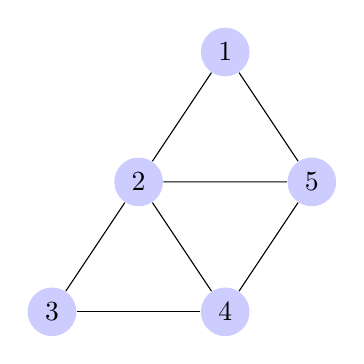
\begin{tikzpicture}
% \label{fig:graph}
  [scale=.55,auto=left,every node/.style={circle,fill=blue!20}]
  \node (n1) at (6, 6) {1};
  \node (n2) at (4,3)  {2};
  \node (n3) at (2,0) {3};
  \node (n4) at (6,0)  {4};
  \node (n5) at (8,3)  {5};
  \foreach \from/\to in {n4/n5,n5/n1,n1/n2,n2/n5,n2/n3,n3/n4,n4/n2}
    \draw (\from) -- (\to);
\end{tikzpicture}
% \label{fig:tree}
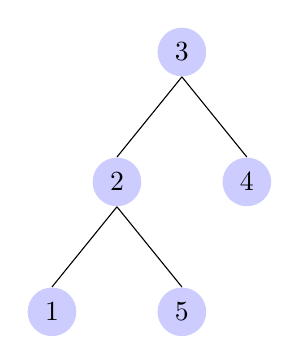
\begin{tikzpicture}
[scale=1.1,auto=left,every node/.style={circle,fill=blue!20}]
\node{3}
    child{ node{2}
        child{ node {1}}
        child{node {5}}
    }
    child{node{4}};
\end{tikzpicture}
}{%
  \caption{graph and spanning tree}%
}
\capbtabbox{%
  
  
\begin{tabular}{
>{\columncolor[HTML]{C0C0C0}}l |
>{\columncolor[HTML]{000000}}l |l|lllll}
\cline{2-3}
\cellcolor[HTML]{000000}{\color[HTML]{FFFFFF} 3:} & \cellcolor[HTML]{FFFFFF}{\color[HTML]{333333} 2} 
& \cellcolor[HTML]{FFFFFF}{\color[HTML]{333333} 4} &  &                                                                       &  & \begin{tabular}[c]{@{}l@{}}d(2)=1\\ d(4)=1\end{tabular} & \begin{tabular}[c]{@{}l@{}}$\pi$(2)=3\\ $\pi$(4)=3\end{tabular} \\ \cline{2-5}
{\color[HTML]{000000} 2:}                         & \cellcolor[HTML]{FFFFFF}1                        & \cellcolor[HTML]{FFFFFF}5                        & \multicolumn{1}{l|}{\cellcolor[HTML]{000000}{\color[HTML]{FFFFFF} 3}} & \multicolumn{1}{l|}{\cellcolor[HTML]{C0C0C0}{\color[HTML]{000000} 4}} &  & \begin{tabular}[c]{@{}l@{}}d(1)=2\\ d(5)=2\end{tabular} & \begin{tabular}[c]{@{}l@{}}$\pi$(1)=2\\ $\pi$(5)=2\end{tabular} \\ \cline{2-5}
{\color[HTML]{000000} 4:}                         & {\color[HTML]{FFFFFF} 2}                         & \cellcolor[HTML]{C0C0C0}5                        & \multicolumn{1}{l|}{\cellcolor[HTML]{000000}{\color[HTML]{FFFFFF} 3}} &                                                                       &  &                                                         &                                                             \\ \cline{2-4}
{\color[HTML]{000000} 1:}                         & {\color[HTML]{FFFFFF} 2}                         & \cellcolor[HTML]{C0C0C0}5                        &                                                                       &                                                                       &  &                                                         &                                                             \\ \cline{2-4}
{\color[HTML]{000000} 5:}                         & {\color[HTML]{FFFFFF} 4}                         & \cellcolor[HTML]{000000}{\color[HTML]{FFFFFF} 1} & \multicolumn{1}{l|}{\cellcolor[HTML]{000000}{\color[HTML]{FFFFFF} 2}} &                                                                       &  &                                                         &                                                             \\ \cline{2-4}
\end{tabular}
  
}{%
  \caption{d and $\pi$ values of each step}%
}
\end{floatrow}
\end{figure}

To use BST in this graph, a spanning tree rooted at $3$ is formed 
% as Figure~\ref{fig:tree}. 
\end{homeworkProblem}

%----------------------------------------------------------------------------------------------
%	PROBLEM 2
%----------------------------------------------------------------------------------------------
\begin{homeworkProblem}

The spanning tree is 

\begin{figure}[ht!]
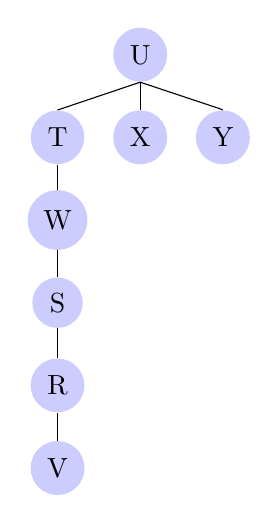
\begin{tikzpicture}
[scale=0.7,auto=left,every node/.style={circle,fill=blue!20}]
\node{U}
    child{ node{T}
        child{ node {W}
            child{ node {S}
                child{ node {R}
                    child{ node {V}
                    }
                }
            }
        }
    }
    child{node{X}}
    child{node{Y}};
\end{tikzpicture}
\end{figure}
d(T) = 1, $\pi$(T) = U; d(X) = 1, $\pi$(X) = U; d(Y) = 1, $\pi$(Y) = U; d(W) = 2, $\pi$(W) = T;\\
d(S) = 3, $\pi$(S) = W; d(R) = 4, $\pi$(R) = S; d(V) = 5, $\pi$(V) = R; 
\end{homeworkProblem}

%----------------------------------------------------------------------------------------------
%	PROBLEM 3
%----------------------------------------------------------------------------------------------
\begin{homeworkProblem}
According to the assumption, we don't need to connect all boxers in a spanning tree. 

\begin{lstlisting}[frame=single]
BFS-MASTER(L)
    foreach v in L
        if COLOR(v) = white
            BFS(v)

BFS(v)
    Q = {v}
    type(v) = GOOD
    while Q is not empty
        u <- dequeue(Q)
        parent_type <- type(u)
        for n in ADJ(u)
            if not type(n) = null
                type(u) <- null
            if color(n) = white
                enqueue(n)
                color(n) <- gray
                type(n) <- FLIPRIVAL(parent_type)
            if k in ADJ(u) and k in ADJ(n)
                type(k) = null
        color(u) <- black

FLIPRIVAL(type)
    if type = GOOD 
        return BAD
    else return GOOD //(including null)
\end{lstlisting}

The root type of each spanning tree is GOOD. 
Between each level, the type is the opposite (this feature is similar to Red Black tree), 
changed by FLIPRIVAL(type). If there's an edge between 2 nodes on the same level, then we remove
both types. Their children would be initiated with GOOD. \\

When there's a circle in the graph, the types of all these nodes in this circle are undecidable. 
Instead of void the types of all nodes, we can only remove the type of one node as undecidable in 
order to let others keep their types. 
Once the new spanning tree has node i and a rivalry between node i and node j, where node j in a 
a another spanning tree and its type is already set, then node i is undecidable so its type is 
set to null. 

\end{homeworkProblem}

%----------------------------------------------------------------------------------------------
%	PROBLEM 4
%----------------------------------------------------------------------------------------------
\begin{homeworkProblem}
DFS performs in Figure~\ref{fig:dfs4} in Page~\pageref{fig:dfs4}.

\begin{figure}[ht!]
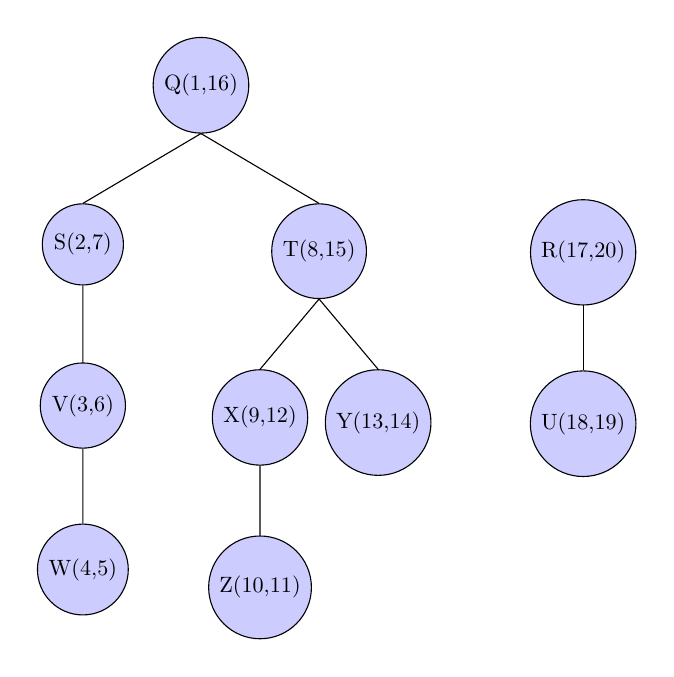
\begin{tikzpicture}[
>=stealth', semithick, node distance=1cm, level distance=15mm, 
    level/.style={sibling distance=30mm/#1},
    round/.style = {draw, circle, fill=blue!20, scale=0.8,minimum height=1cm},
    every node/.style={circle, draw, fill=none, anchor=north},
]
    
\node (tree 1) [draw=none, rectangle] {\tikz{%
\node (tree 1) [round] {Q(1,16)}
    child{ node[round] {S(2,7)}
        child{ node[round] {V(3,6)}
            child{ node[round] {W(4,5)}
            }
        }
    }
    child{ node[round] {T(8,15)}
        child{ node[round] {X(9,12)}
            child{ node[round] {Z(10,11)}
            }
        }
        child{ node[round] {Y(13,14)}}
    }
}};

\node (tree 2) [draw=none, rectangle, right=of tree 1] {\tikz{%
\node (tree 2) [round] {R(17,20)}
    child{ node[round] {U(18,19)}
    }
}};

\end{tikzpicture}
\caption{dfs for B}
\label{fig:dfs4}
\end{figure}



\end{homeworkProblem}

%----------------------------------------------------------------------------------------------
%	PROBLEM 5
%----------------------------------------------------------------------------------------------
\begin{homeworkProblem}
See the result in Figure~\ref{fig:topsort5} in Page~\pageref{fig:topsort5}. 
Represent (distance time, finishing time) as a pair, the result linked list is 
[P(27,28), N(21,26), O(22,25), S(23,24), M(1,20), R(8,19), Y(11,18), V(12,17), W(13,16),
Z(14,15), U(9,10), Q(4,7), X(2,3)]

\begin{figure}[ht!]
\centering
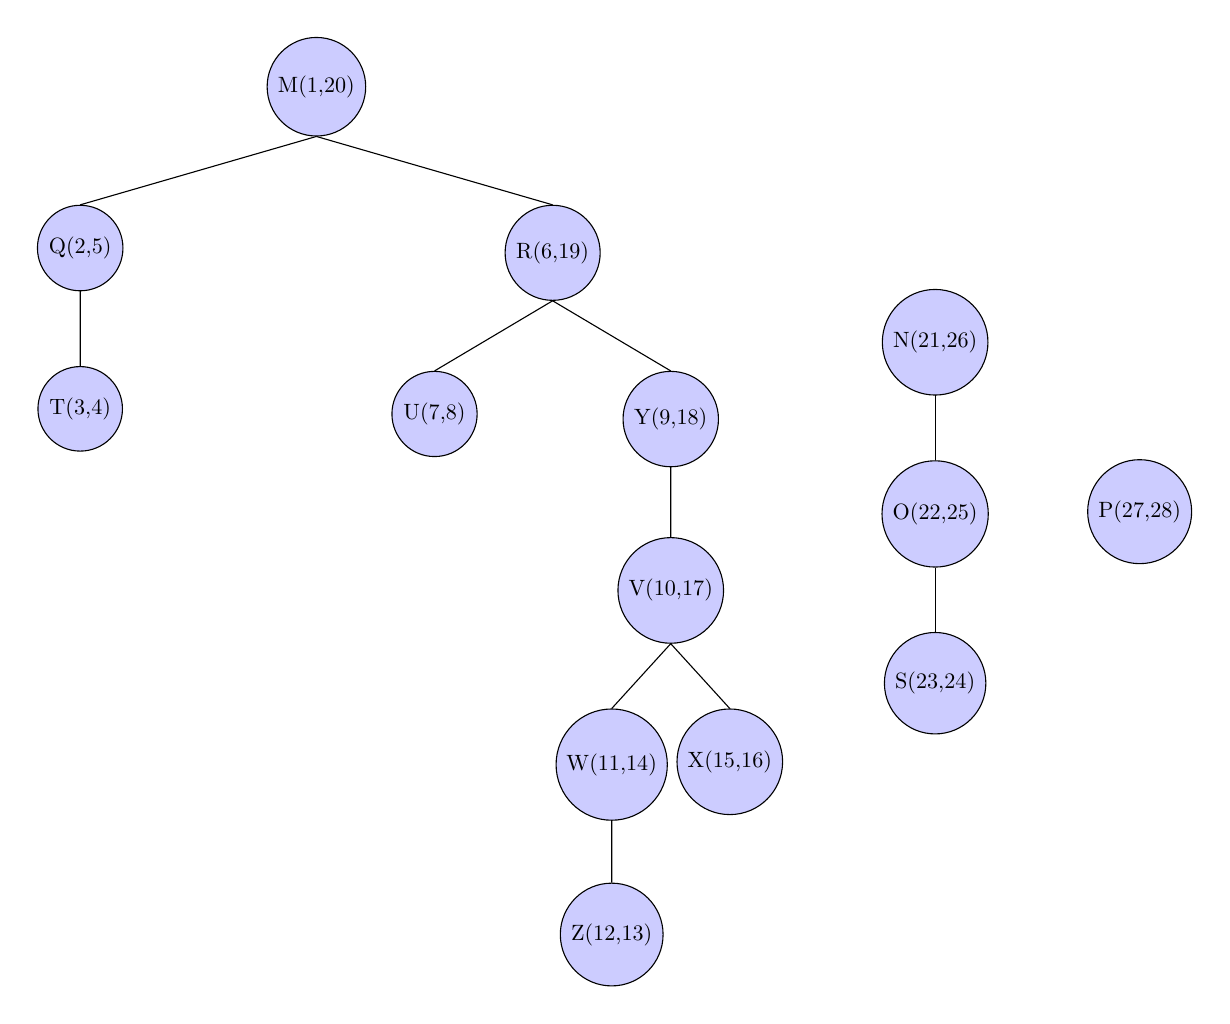
\begin{tikzpicture}[
>=stealth', semithick, node distance=1cm, level distance=15mm, 
    level/.style={sibling distance=60mm/#1},
    round/.style = {draw, circle, fill=blue!20, scale=0.8,minimum height=1cm},
    every node/.style={circle, draw, fill=none, anchor=north},
]
    
\node (tree 1) [draw=none, rectangle] {\tikz{%
\node (tree 1) [round] {M(1,20)}
    child{ node[round]{Q(2,5)}
        child{ node[round]{T(3,4)} }
    }
    child{ node[round]{R(6,19)}
        child{ node[round]{U(7,8)} }
        child{ node[round]{Y(9,18)} 
            child{ node[round]{V(10,17)} 
                child{ node[round]{W(11,14)}
                    child{ node[round]{Z(12,13)} }
                }
                child{ node[round]{X(15,16)} }
            }
        }
    };
}};

\node (tree 2) [draw=none, rectangle, right=of tree 1] {\tikz{%
\node (tree 2) [round] {N(21,26)}
    child{ node[round]{O(22,25)} 
        child{ node[round]{S(23,24)} }
    };
}};

\node (tree 3) [draw=none, rectangle, right=of tree 2] {\tikz{%
\node (tree 3) [round] {P(27,28)}{};
}};
\end{tikzpicture}
\caption{Topsort for C}
\label{fig:topsort5}
\end{figure}

The list should be [P N O S M R Y V X W Z U Q T]. 
\end{homeworkProblem}

%----------------------------------------------------------------------------------------------
%	PROBLEM 6
%----------------------------------------------------------------------------------------------
\begin{homeworkProblem}
\begin{enumerate}[(a)]
    \item When a leaf node is reached, the game stops. 
          The number of steps is finite. The graph is unidirectional so no way back.
          There's no cycle in DAG. $n - 1$ steps can be reached when the height
          of the $n$-node spanning tree is $n-1$, meaning all nodes in 1 path. \\
          
          In a DAG, for each vertex $v$, there's a spanning tree rooted at $v$ so a leaf node 
          would be reached at most $n - 1$ steps because its maximum height is $n - 1$.
    \item We can extend the notion that the leaf node {\tt z} would be {\tt VALUE[z]} = Dos, 
          {\tt VALUE[PARENT(z)]} = Uno. 
          We mark the linked list from the end with {\tt VALUE[L(end)]} = Dos, 
          {\tt VALUE[L(end - 1]} = Uno,
          {\tt VALUE[L(end - 2)]} = Dos until the beginning {\tt z}.    
          
          But if the height of a node's children are different, let's say,
          node $n: u, v$ has 2 branches, $u: t$, $t: z$, $v: q$, $u$ is height 1 but $v$ is height 0.
          If Dos move to $v$, Dos win. If Dos move to $u$, Uno moves to $z$ and Uno win. 
          {\tt VALUE[n]} is undecidable so {\tt VALUE[n]} is null. 
          See Figure~\ref{fig:nim} in Page~\pageref{fig:nim}.
          
          
\begin{figure}[h!]
\centering
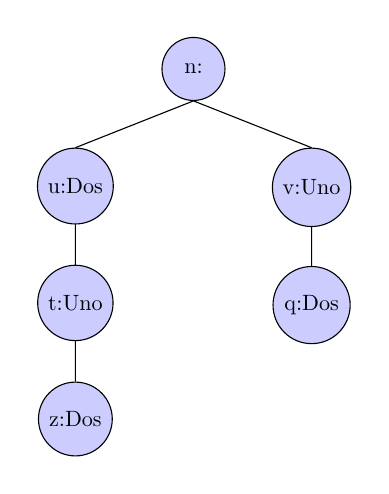
\begin{tikzpicture}[
>=stealth', semithick, node distance=1cm, level distance=10mm, 
    level/.style={sibling distance=30mm/#1},
    round/.style = {draw, circle, fill=blue!20, scale=0.8,minimum height=1cm},
    every node/.style={circle, draw, fill=none, anchor=north},
]
    
\node (tree 1) [draw=none, rectangle] {\tikz{%
\node (tree 1) [round] {n:}
    child{ node[round]{u:Dos}
        child{ node[round]{t:Uno} 
            child{ node[round]{z:Dos} }
        }
    }
    child{ node[round]{v:Uno}
        child{ node[round]{q:Dos} }
    }
}};
\end{tikzpicture}
\caption{Sample Nim}
\label{fig:nim}
\end{figure}


    \item The running time would be ($v+e$) for a $n$ node graph. 
\begin{lstlisting}[frame=single]
DFS-VISIT(v)
    color(v) <- gray
    time++
    d(v) <- time
        
    foreach u in ADJ(v)
        if color(u) = white
            pi(u) <- v
            DFS-VISIT(u)
    
    if ADJ(v) empty
        value(v) <- Dos
    else if foreach u in ADJ(v), value(u) are same
        value(v) <- swap_value(u)
        
    color(v) <- black
    time++
    f(v) <- time

swap_value(v)
    if value(v) = Uno
        return Dos
    else return Uno
\end{lstlisting}

\end{enumerate}



\end{homeworkProblem}


% \begin{lstlisting}[frame=single]
% \end{lstlisting}

% \begin{enumerate}[a.]
%     \item 
        %   
% \end{enumerate}

% \begin{figure}[h!]
%     \centering
%     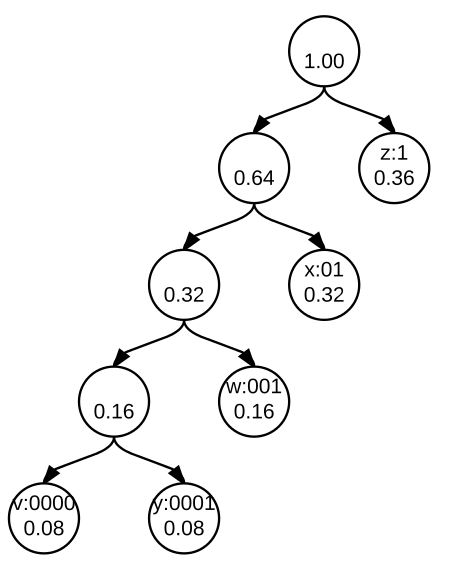
\includegraphics[scale=0.4]{hw8/2.png}
%     \caption{}
%     \label{fig:forz}
% \end{figure} 

% Figure~\ref{fig:tree} on Page~\pageref{fig:tree}.
% \begin{figure}[h!]
%     \centering
%     \subfigure[]{\label{}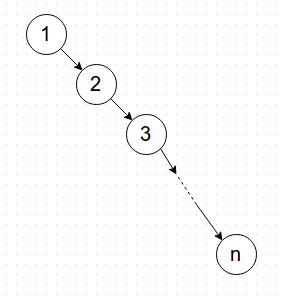
\includegraphics[scale=0.4]{hw6/51.png}}
%     \subfigure[]{\label{}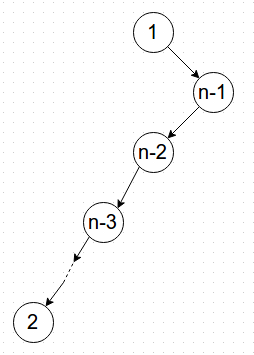
\includegraphics[scale=0.4]{hw6/52.png}}
%     \caption{}
%     \label{fig:tree}
% \end{figure} 

% \begin{tikzpicture}
%   [scale=.6,auto=left,every node/.style={circle,fill=blue!20}]
%   \node (n1) at (6, 6) {1};
%   \node (n2) at (4,3)  {2};
%   \node (n3) at (2,0) {3};
%   \foreach \from/\to in {n1/n2,n2/n3}
%     \draw (\from) -- (\to);
% \end{tikzpicture}

% \begin{tikzpicture}[
% >=stealth', semithick, node distance=1cm, level distance=15mm, 
%     level/.style={sibling distance=30mm/#1},
%     round/.style = {draw, circle, fill=blue!20, scale=0.8,minimum height=1cm},
%     every node/.style={circle, draw, fill=none, anchor=north},
% ]
% \node (tree 1) [draw=none, rectangle] {\tikz{%
% \node (tree 1) [round] {Q(1,16)}
%     child{ node[round] {S(2,7)} }
% }};
% \node (tree 2) [draw=none, rectangle, right=of tree 1] {\tikz{%
% \node (tree 2) [round] {R(17,20)}
% }};
% \end{tikzpicture}

\end{document}